\chapter{Tabela de Erros} \label{tabelaErros}

Como sabe-se sistemas apresentam restrições quanto as entradas fornecidas de modo a realizar determinadas atividades. Na HP-12C entradas inválidas produzem erros que são apresentados ao usuário através de um código no formato \textbf{ERROR d+}, onde d+ indica um ou mais dígitos. Esse formato dificulta o entendimento por parte do usuário do motivo que levou ao erro, ou seja, o usuário necessita ter em mãos o manual da calculadora que explicita o significado do código visualizado.

Nesse sentido, buscou-se fazer uso das facilidades que o dispositivo computacional em foco oferece de modo a melhorar a usabilidade do sistema. Para isso foi realizado um mapeamento dos códigos de erros encontrados nos cálculos financeiros na HP-12C para mensagens de texto que explicitem melhor o problema encontrado. 

Como a aplicação desenvolvida é composta de uma biblioteca financeira que é utilizada pela aplicação calculadora financeira, optou-se por realizar dois mapeamentos: um das mensagens que são geradas pelos cálculos financeiros da biblioteca e outro das mensagens que são geradas por estados inconsistentes na calculadora. Tais mapeamentos estão presentes nas tabelas \ref{tabErros1} e \ref{tabErros2}.

\begin{figure}[!h]
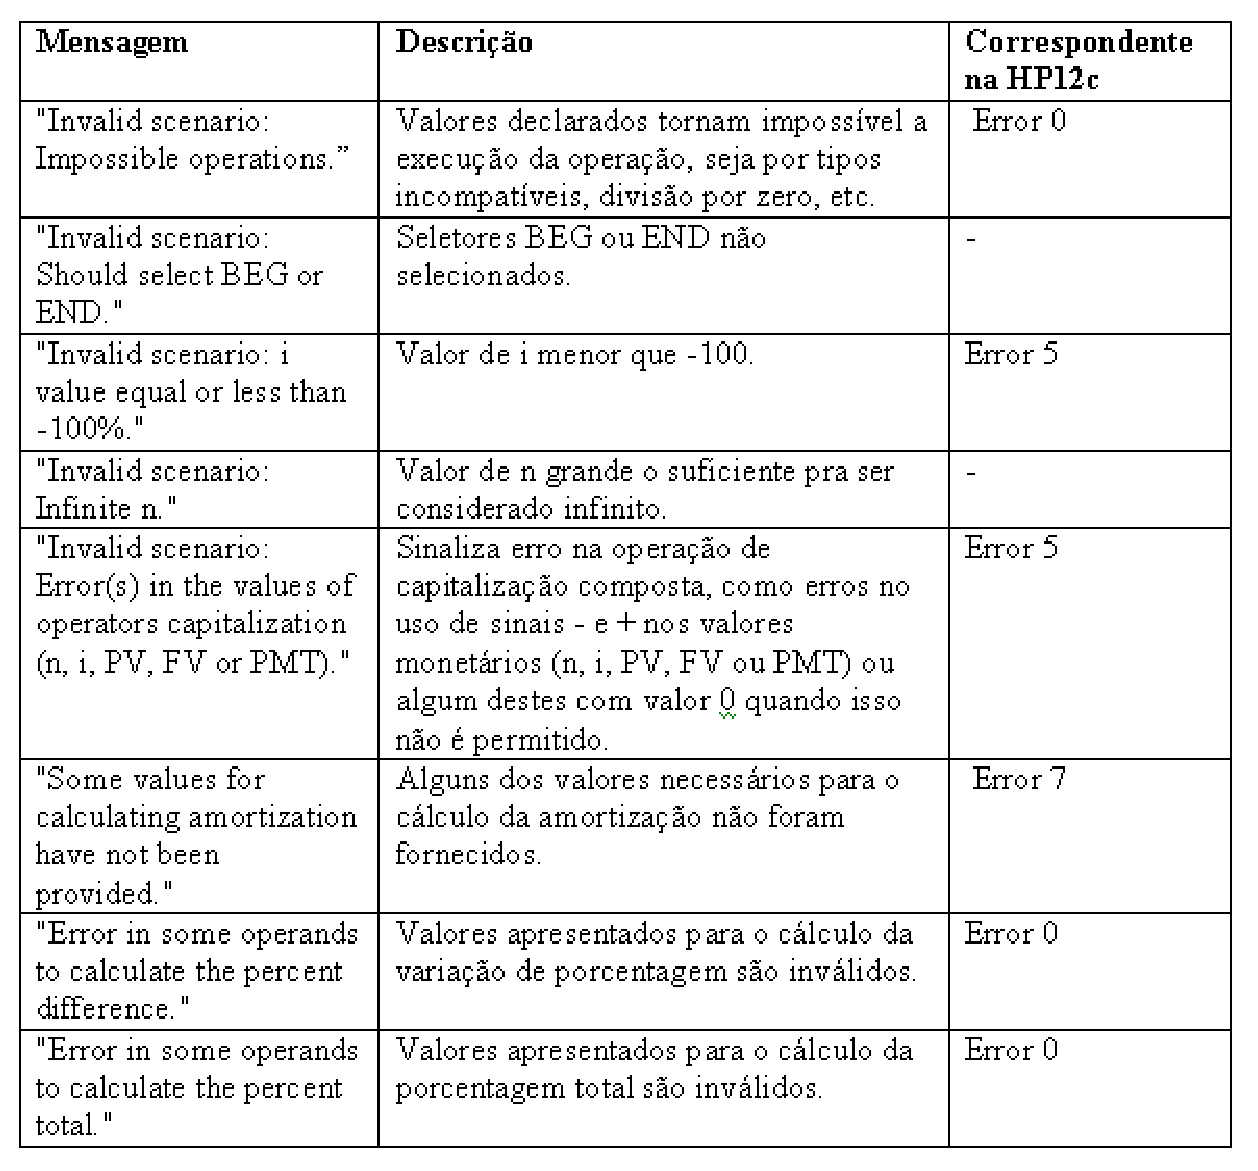
\includegraphics[scale = .7]{tabErro1.eps}
%  \includegraphics[scale=0.5]{bigchart.eps}
\caption{\it Mapeamento de Erros da Biblioteca}
\label{tabErros1} 
\end{figure}

\begin{figure}[!h]
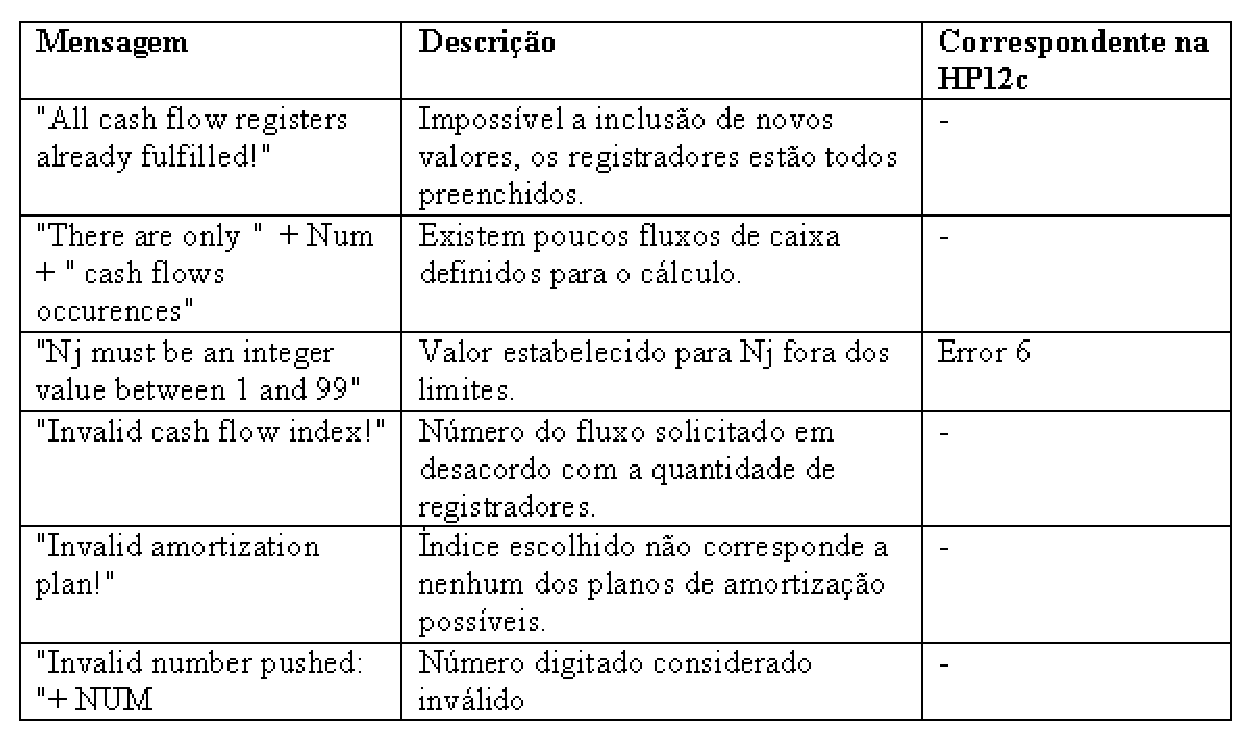
\includegraphics[scale = .7]{tabErro2.eps}
\caption{\it Mapeamento de Erros da Calculadora}
\label{tabErros2}
\end{figure}